\label{monitoramento_servicos}

Neste capítulo são apresentadas informações decorrentes da realização do monitoramento do barramento de serviços utilizando o Protocolo \acrshort{SNMP}. Na Seção \ref{recursos_monitoramento} é a apresentado o monitoramento dos recursos do barramento de serviços. Na Seção \ref{integracao_snmp} são apresentados alguns detalhes para a implantação do protocolo \acrshort{SNMP}. Na Seção \ref{metricas_monitoramento} são apresentadas as métricas adotadas para a realização do monitoramento do barramento. Na Seção ('\ ref') é apresentado o ......

\section{Monitoramento dos recursos do barramento de serviços}%
\label{recursos_monitoramento}

O \acrshort{CPD} da \acrshort{UnB} adotou como solução para a modernização, migração dos sistemas e tecnologia a implementação de uma arquitetura orientada a serviços, que vem sendo bastante utilizada principalmente para criação de serviços (\textit{web services}). A implementação dos serviços tem aumentado, devido a flexibilidade definida na arquitetura e o aumento da demanda para a realização de integração de sistemas, além da curva de aprendizagem ser alta. Com a implementação e disponibilização de  vários serviços, monitorar e acompanhar o funcionamento, tem se tornado uma tarefa que tem demandado um grande esforço das equipes de 
desenvolvimento do \acrshort{CPD}. O monitoramento do barramento de serviços da \acrshort{UnB} é realizado de três formas conhecidas, uma por meio do \textit{Log} de arquivos gerado pelo próprio barramento, onde as informações de registros do \textit{Log} são coletadas e apresentadas em um \textit{dashboard}, que pode ser visualizado na figura \ref{fun:fig:dashboardS} \cite{filgueirasmonitoramento}, outra por meio de serviços (\textit{web services}) providos pelo barramento conforme a figura \ref{fun:fig:memoriaEMS}, além da nativa que é disponibilizada pela empresa que mantém e gerencia a linguagem Erlang, esse monitoramento é realizado pelo denominado \textit{Observer} que dispõe de elementos gráficos como apresentado na figura \ref{fun:fig:observer} que possibilita observar as características dos sistemas desenvolvidos em Erlang \cite{ericssonAB2002-2019}. 

\begin{figure}[h!]
	\begin{center}
	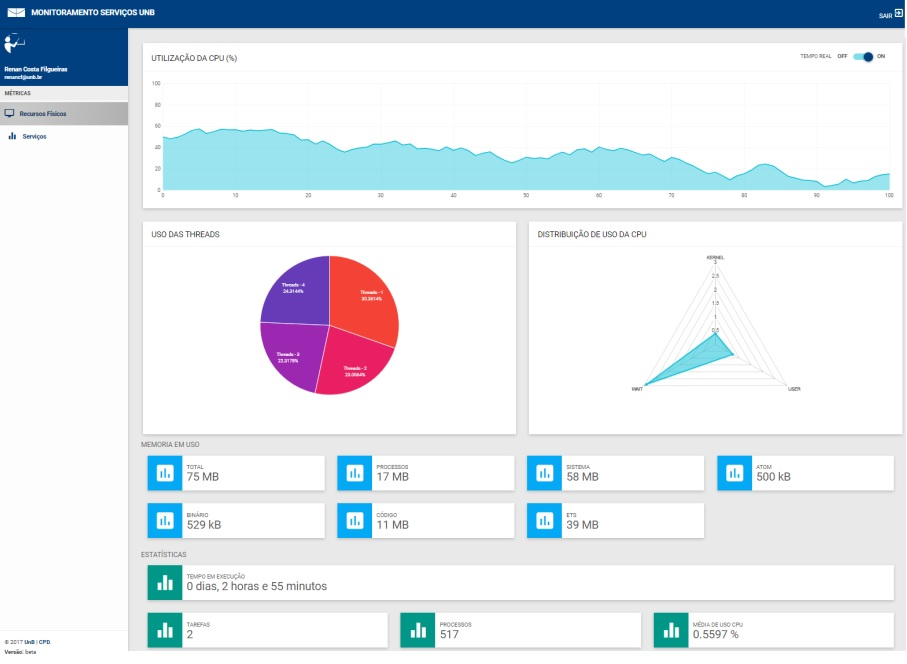
\includegraphics[scale = 0.70]{img/dashboard.jpg}
		\caption{\textit{Dashborad} de monitoramento \cite{filgueirasmonitoramento}.}
		\label{fun:fig:dashboardS}
	\end{center}
\end{figure}

Este trabalho inclui uma nova forma de monitoramento para o barramento de serviços, esse monitoramento difere dos demais pelo modo de atuação, onde o foco é monitorar o funcionamento dos recuros que o barramento de serviços provém, desde o recurso responsável pelo registro das informações de \textit{Log} passando pelo os recursos que executam os processos de autenticação e autorização até o recurso responsável pelo recebimento e transmissão de requisições. Devido a escolha e definição desse novo modo de monitorar os recursos do barramento foi incluída também a necessidade da realização do monitoramento de serviços na mesma plataforma que os sistemas e ativos de rede da \acrshort{UnB} são monitorados, tentando garantir o monitoramento dos serviços, sistemas e ativos de rede em uma única plataforma que permitisse apresentar o funcionamento dessas aplicações ou em casos eventuais notificar sobre possíveis falhas ou problemas. Diante desse cenário optou-se por definir um meio de comunicação onde a ferramenta de monitoramento, mantida e gerenciada pelo \acrshort{CPD} da \acrshort{UnB} pudesse receber as informações para a realização do monitoramento do barramento de serviços, por meio de um protocolo, neste trabalho o protocolo utilizado para a realização da comunicação e permitir a integração das ferramentas foi o protocolo \acrshort{SNMP}. A escolha do protocolo para a realização do monitoramento busca um meio para tentar garantir a implantação e integração das aplicações com baixo acoplamento, onde a importância é a preservar a uniformidade na comunicação das aplicações por meio de um protocolo, principalmente quando houver alguma mudança de ferramenta de monitoramento, no mercado as principais ferramentas de monitoramento se comunicam e permitem a transmissão de dados e informações por meio do protocolo \acrshort{SNMP}, ou seja independente de ferramenta o serviços de monitoramento seria facilmente plugado e configurado em ferramentas de monitoramento que utilização o protocolo \acrshort{SNMP} como meio de comunicação.      

\begin{figure}[h!]
	\begin{center}
	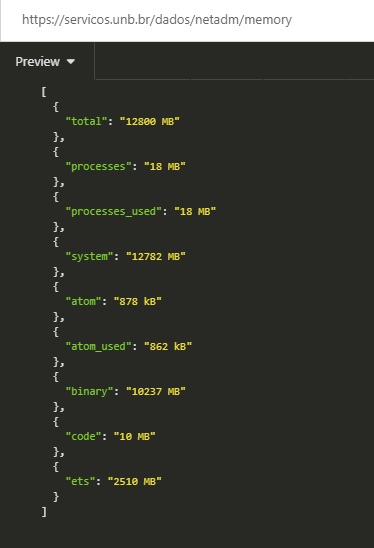
\includegraphics[scale = 0.90]{img/monitoramentoEMS.jpg}
		\caption{Serviço de consulta de utilização dos recursos de memória do Erlangms.}
		\label{fun:fig:memoriaEMS}
	\end{center}
\end{figure}

\begin{figure}[h!]
	\begin{center}
	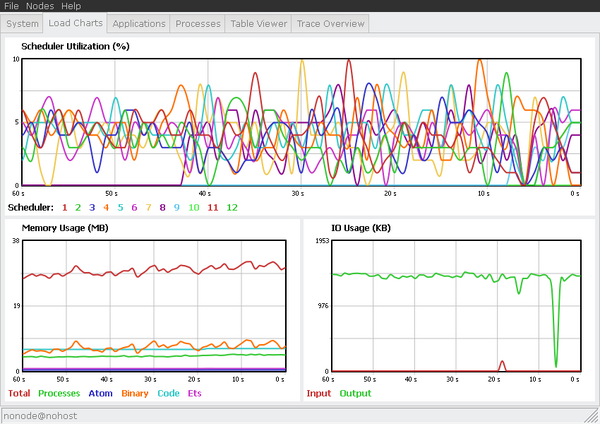
\includegraphics[scale = 0.70]{img/observerGo.jpg}
		\caption{Interface gráfica do \textit{Observer}.}
		\label{fun:fig:observer}
	\end{center}
\end{figure}

\subsection{Execução do monitoramento}

A execução do monitoramento é inciada com a integração das aplicações, ou seja quando o barramento de serviços está em funcionamento, o agente de monitoramento está ativo, assim como a ferramenta de monitoramento está ligada e configurada em modo passivo para receber as informações que são transmitidas de modo a permitir a realização do monitoramento. Para representar a execução do monitoramento foi criado um \textit{design} que pode ser visualizado na figura \ref{fun:fig:arqtProjeto}. O monitoramento é realizado por meio de dados gerados por serviços provenientes do barramento de serviços, esse dados possuem identificação e valores incrementais de contagem. Em seu funcionamento o barramento de serviços pode incrementar ou decrementar informações de contagem dependendo do serviço utilizado, normalmente o valor é incrementado, quando o valor a ser monitorado é coletado, o mesmo é enviado ao agente de monitoramento, o agente de monitoramento tem a responsabilidade de realizar o envio dessa informação, realizando a comunicação com a ferramenta de monitoramento por meio do protocolo \acrshort{SNMP}, a informação transmitida poderá ser visualizada de modo personalizado e configurado na ferramenta de monitoramento, que dependendo da configuração poderá apresentar itens de serviços cadastrados com os status, "Ok" \ para serviços que estejam funcionado normalmente, "\textit{Warning}" \  para serviços que estejam apresntando algo incomum em seu funcionamento e "\textit{Critical}" \ para serviços que estejam apresentando anormalidade ou realmente estejam indisponíveis.	 

\begin{figure}[h!]
	\begin{center}
	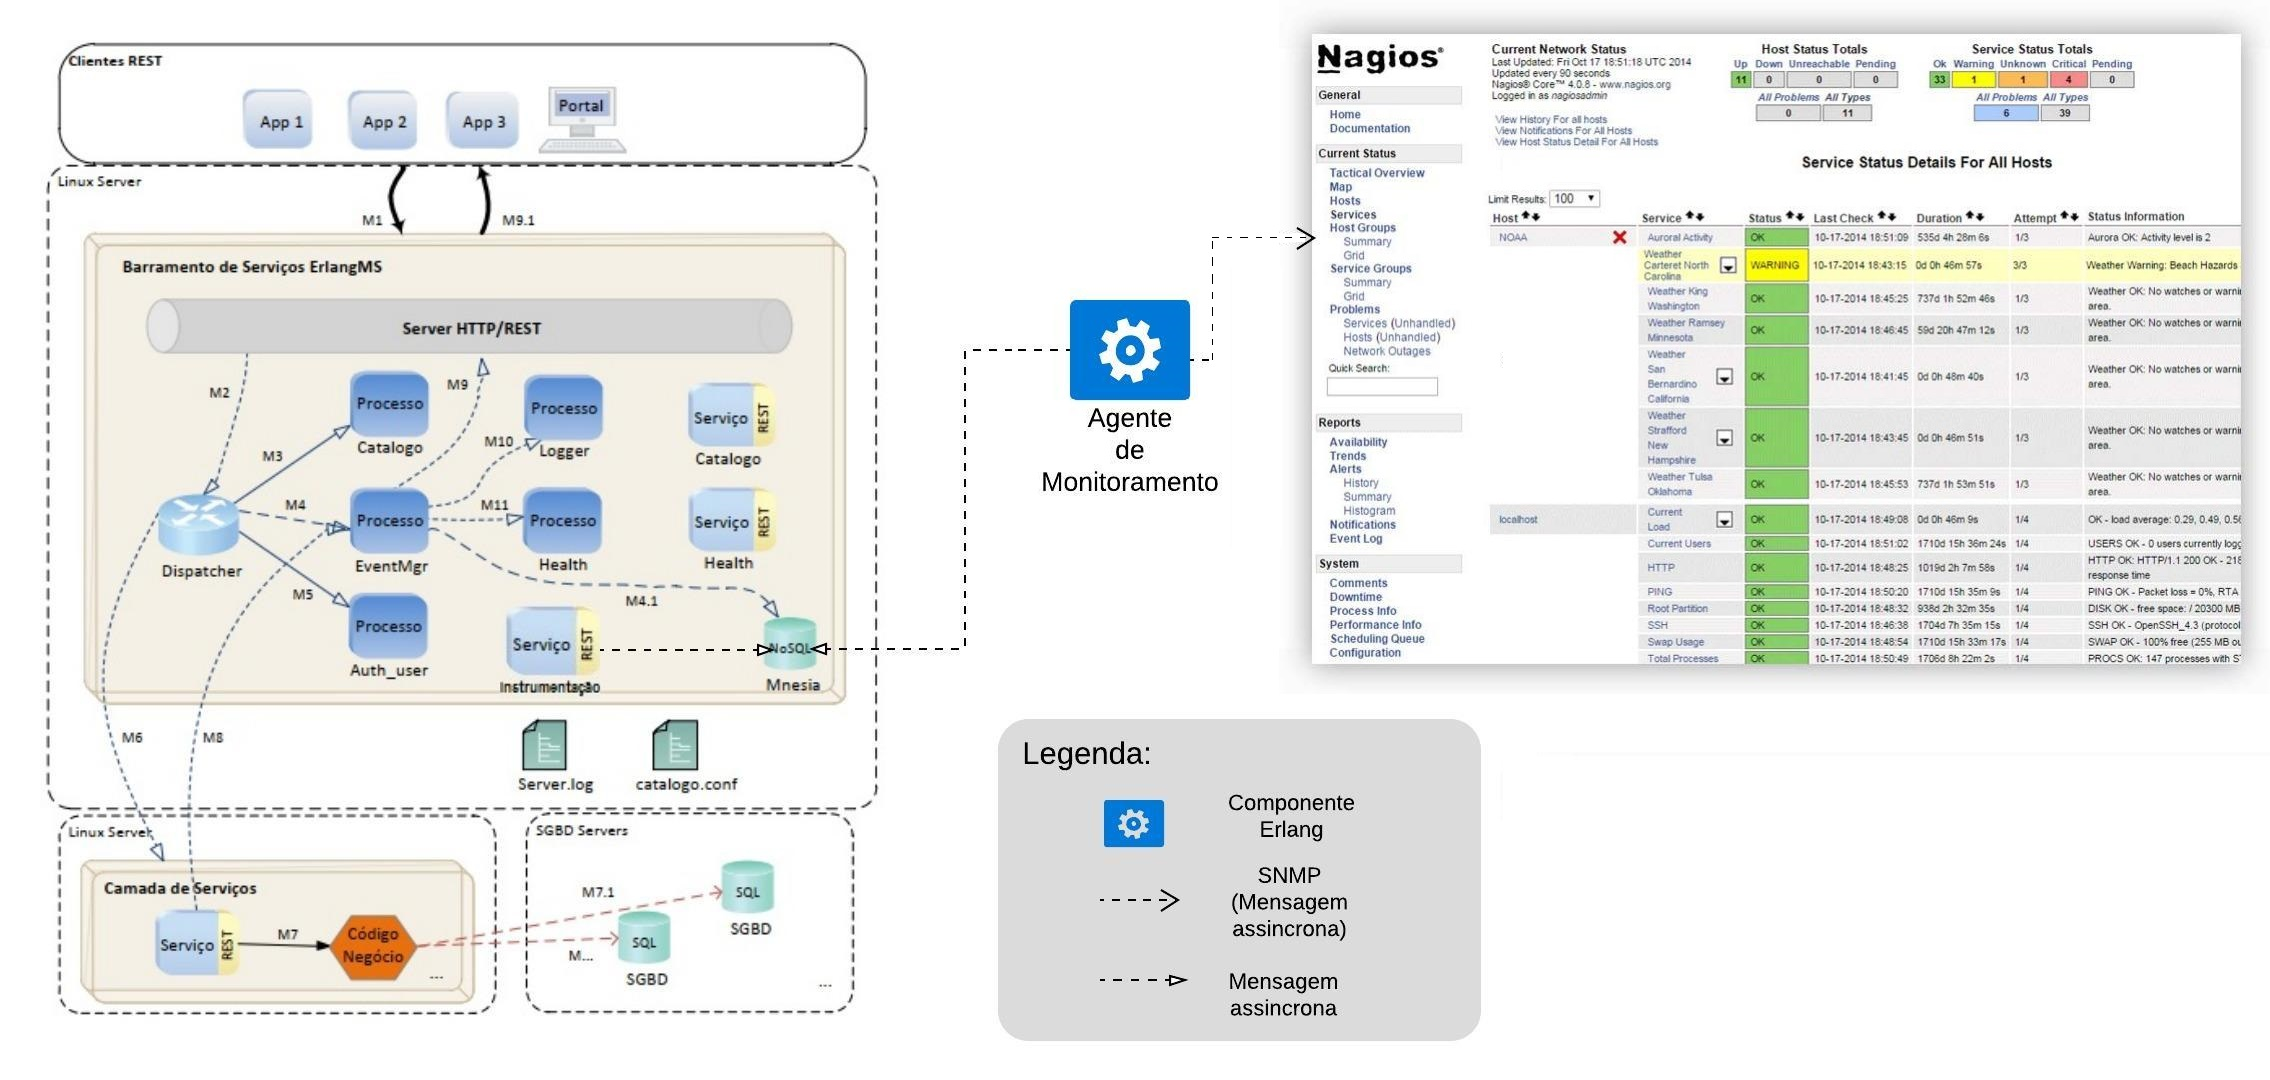
\includegraphics[scale = 0.45]{img/arqtProjeto.jpeg}
	\caption{\textit{Design} da integração das ferramentas para o monitoramento.}
	\label{fun:fig:arqtProjeto}
	\end{center}
\end{figure}



\subsection{Execução do agente de monitoramento}

Para a realização da integração do barramento de serviços e a ferramenta de monitoramento por meio do protocolo \acrshort{SNMP} é utilizado um agente de monitoramento que gerencia a comunicação e transmissão dos dados que são monitorados. O projeto dispõem  da utilização de um agente para a coleta e transmissão desses dados, o agente é originário da aplicação Exometer que é um pacote que permite a instrumentação de aplicações desenvolvidas na linguagem de codificação Erlang, possibilitando que alguns dados do sistema sejam exportados para um grande e variado número de ferramentas de monitoramento disponíveis no mercado\cite{exometer_core}, nesse projeto diante de um dos itens do objetivo específico descrito na seção \ref{objetivos_especificos} optou-se por utilizar o modulo que permite e realizar a transmissão dos dados por meio do protocolo \acrshort{SNMP}. O Exometer cumpre os requisitos definidos na \acrshort{RFC} 1157 que descreve sobre os procedimentos arquiteturais de implementação e implantação do protocolo \acrshort{SNMP}, os pontos fortes do Exometer são, a criação das \acrshort{MIBs} que são geradas dinamicamente em tempo de execução, para a criação das \acrshort{MIBs} que são utilizadas no monitoramento necessita-se de uma estrutura base, essa estrutura poderá ser visualizada na figura \ref{fun:fig:MIBSNMP} e considerada também com um ponto importante é a fácil configuração do Gerente e Agente \acrshort{SNMP}, onde simplesmente você pode registrar em um dos arquivos de configuração o servidor(aplicação de monitoramento) que receberá as informações do monitoramento por meio de \textit{TRAPs} enviados pelo agente \acrshort{SNMP}, as configurações desse arquivo poderá ser visualizada na figura \ref{fun:fig:enderecoAgenteSNMP}. O Exometer foi a aplicação que permitiu a integração das aplicações de um modo prático, visto que a estrutura de um arquivo MIB normalmente já vem configurada com informações especificas e estáticas o que impossibilitaria ou reduziria bastante o escopo de serviços que poderiam ser utilizados para realizar o monitoramento de serviços do barramento. 

\begin{figure}[h!]
	\begin{center}
	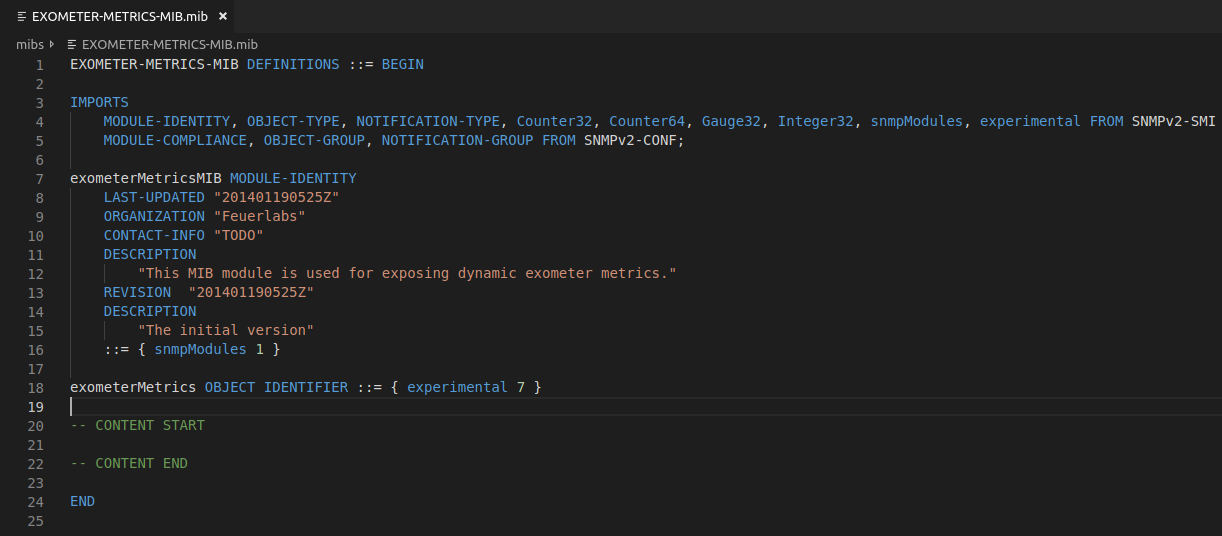
\includegraphics[scale = 0.50]{img/MIBSNMP.png}
	\caption{Estrutura base, arquivo MIB do Exometer.}
	\label{fun:fig:MIBSNMP}
	\end{center}
\end{figure}

\begin{figure}[h!]
	\begin{center}
	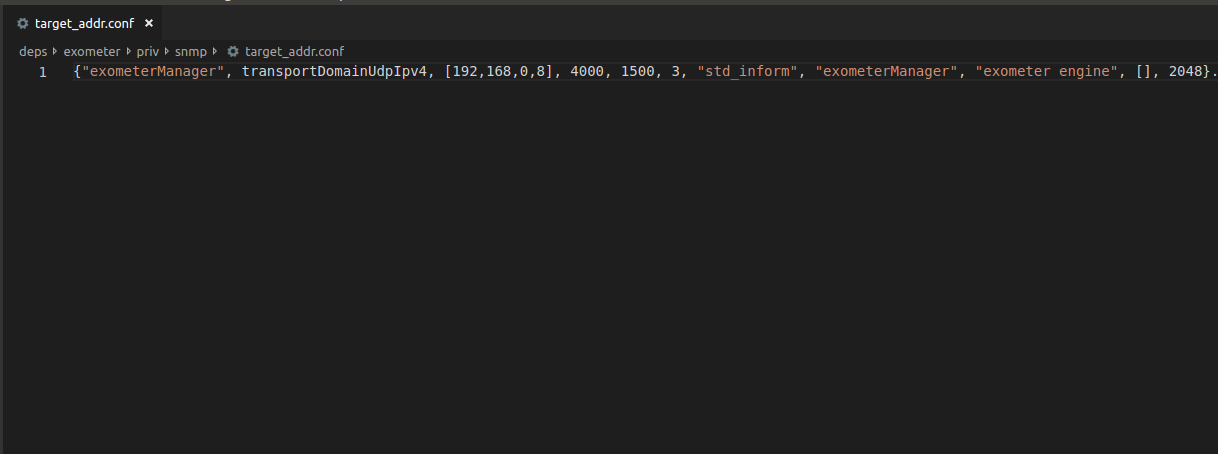
\includegraphics[scale = 0.50]{img/enderecoEnvioAgente.png}
	\caption{Configuração do servido de destino, para o envio de \textit{TRAPs}.}
	\label{fun:fig:enderecoAgenteSNMP}
	\end{center}
\end{figure}

%%%%%%%%%%%%%%%%%%%%%%%%%%%%%%%%%%%%%%%%%%%%%%%%%%%%%%%%%%%%%%%%%%%%%%%%%%%%%

\section{Funcionamento do protocolo \acrshort{SNMP}}
\label{integracao_snmp}
O \acrshort{SNMP} é o protocolo utilizado para o monitoramento de dispositivos conectados em rede. O \acrshort{CPD} da \acrshort{UnB} para o monitoramento dos ativos de rede utiliza-o por meio de ferramentas que recebem informações desse protocolo, no entanto as ferramentas e informações fornecidas para o monitoramento servem apenas para o controle da infraestrutura de rede e servidores de aplicação, não gerenciando por exemplo, o funcionamento dos sistemas, serviços e também pode se dizer a ausência de verificação da saúde das aplicações. Este trabalho implementa e implanta soluções capazes de fornecer e subsidiar recursos que possibilitem o monitoramento e a integração com a ferramenta de monitoramento do \acrshort{CPD} da \acrshort{UnB} que vem durante alguns anos adotando o Nagios\textsuperscript{\textregistered} com a ferramenta de monitoramento dos seus ativos de rede, o \acrshort{SNMP} tem como característica a singularidade na comunicação o que possibilita a escolha de outras ferramentas, serviços ou aplicações que conversem em \acrshort{SNMP}. 

O funcionamento do monitoramento por meio do protocolo \acrshort{SNMP} neste trabalho é realizado pelo envio de \textit{TRAPS} a partir da coleta de informações geradas pelo barramento de serviços e enviadas pelo agente, para que o agente funcione é necessária a configuração de um gerente, o gerente funciona como a representação do cliente monitorado e o agente funciona como responsável por enviar as informações desse cliente, na figura \ref{fun:fig:agenteConfig} é apresentada a configuração do agente na aplicação e na figura \ref{fun:fig:gerenteConfig} é exposta a configuração do gerente. 

\begin{figure}[h!]
	\begin{center}
	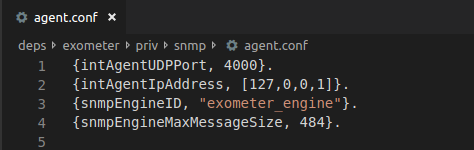
\includegraphics[scale = 0.99]{img/agenteConfig.png}
	\caption{Arquivo de configuração do agente \acrshort{SNMP}.}
	\label{fun:fig:agenteConfig}
	\end{center}
\end{figure}

\begin{figure}[h!]
	\begin{center}
	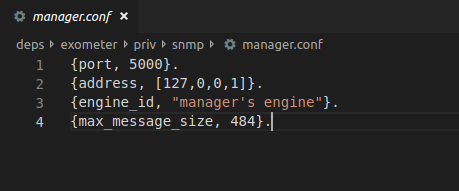
\includegraphics[scale = 0.99]{img/gerenteConfig.png}
	\caption{Arquivo de configuração do gerente \acrshort{SNMP}.}
	\label{fun:fig:gerenteConfig}
	\end{center}
\end{figure}


O \textit{TRAP} é um tipo de alerta ou evento que pode ser transmitido pelo protocolo, na figura \ref{fun:fig:debugTrap} é apresentada a informações de um \textit{TRAP} \acrshort{SNMP} com a verbosidade \textit{debug}. Durante a coletada das informações em tempo de execução e o envio de \textit{TRAPS} pelo agente para a ferramenta do monitoramento é necessária a instalação e configuração para de alguns \textit{plugins}, visto que o Nagios\textsuperscript{\textregistered} trabalha de forma em que é possível a realização do monitoramento ativo e passivo, como informado anteriormente este trabalho aplica o monitoramento passivo, diante desse cenário os \textit{plugins} instalados e configurados são eles:
\begin{itemize}
\item \acrfull{SNMPTT} que é um \textit{plugin} que funciona com um tradutor de \textit{TRAP} \acrshort{SNMP} com diversas opções de saída para a utilização no Nagios Core\textsuperscript{\textregistered} e o Net-SNMP\cite{nagiosCoreSNMPTT}.
\item SNMPTRAPD que é uma aplicação que funciona com o recebimento dos \textit{TRAP} que foram traduzidos pelo \acrshort{SNMPTT} \cite{net_snmptrapd}.
\end{itemize}

\begin{figure}[h!]
	\begin{center}
	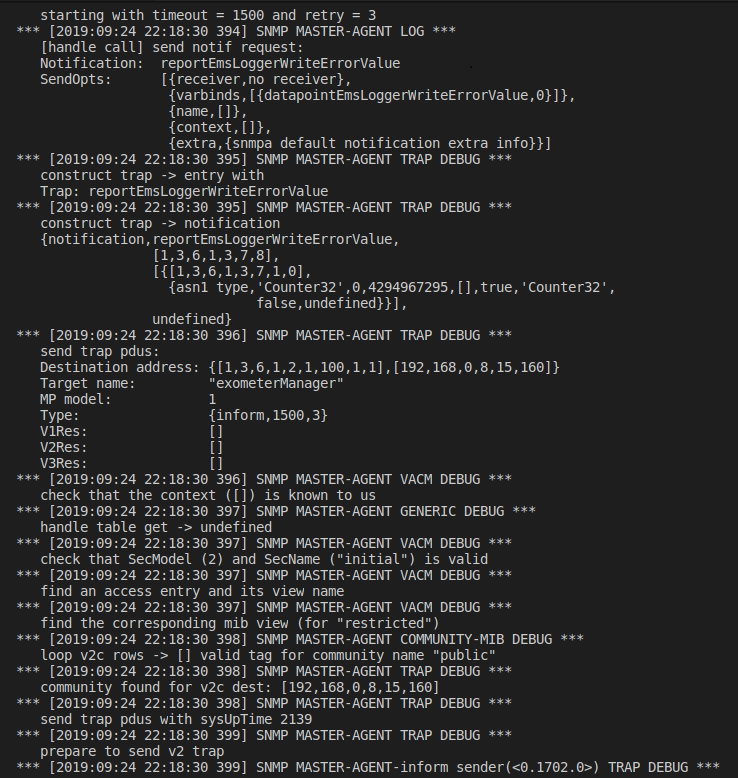
\includegraphics[scale = 0.70]{img/debugTrap.png}
	\caption{Informações do \textit{TRAP}.}
	\label{fun:fig:debugTrap}
	\end{center}
\end{figure}

Com a instalação e configuração realizada do \acrshort{SNMPTT} e SNMPTRAPD foi possível realizar a interceptação das informações enviadas pelo agente \acrshort{SNMP}, cada item com sua especifidade com por exemplo, no \acrshort{SNMPTT} é necessária a configuração das variáveis dos \acrshort{OID}'s  criadas e definidas nas \acrshort{MIBs} do agente, já na configuração SNMPTRAPD é necessário definir quais os \acrshort{OID}'s serão enviados à ferramenta de monitoramento e quais o tipo de informação serão enviadas, poderão ser enviadas informações dos tipos  "Ok", "\textit{Warning}" ,"\textit{Critical}" \ dependendo do \acrshort{OID} e da definição que pode ser facilmente configurada. Desse modo é realizada a integração das ferramentas para a execução do monitoramento, por meio do protocolo \acrshort{SNMP} a comunicação entre o barramento de serviços e o Nagios\textsuperscript{\textregistered} é praticada.  

%%%%%%%%%%%%%%%%%%%%%%%%%%%%%%%%%%%%%%%%%%%%%%%%%%%%%%%%%%%%%%%%%%%%

\section{Definição das métricas de monitoramento}
\label{metricas_monitoramento}

Com a elaboração da integração entre o barramento de serviços e o Nagios\textsuperscript{\textregistered} foi feita a pesquisa na literatura especifica relacionada ao tema métricas de monitoramento para auxiliar a definição do que dever ser monitorado. Após a realização da pesquisa e durante a execução da configuração da ferramenta de monitoramento percebeu-se a necessidade de seguir a estrutura de configuração determinada na ferramenta de monitoramento, ao assumir essa estrutura foi possível detectar que o monitoramento deveria ser executado de um novo modo, implicando na mudança da estratégia de definição para a execução do monitoramento dos recursos do barramento de serviços. Como o monitoramento é realizado em modo passivo é preciso informar na configuração da ferramenta de monitoramento quais as informações serão recebidas, ou seja, mesmo o agente \acrshort{SNMP} do barramento de serviços criando os \acrshort{OID}'s dinamicamente é necessário que estes \acrshort{OID}'s estejam também registrados na ferramenta de monitoramento, nesse momento  não foi possível a realização da implementação de uma solução para automatizar a configuração dinâmica dos \acrshort{OID}'s na ferramenta de monitoramento, mas em um outro momento oportuno essa automatização poderá ser implementada.

Com a restrição imposta pela ferramenta de monitoramento, foi necessário a realização de um estudo no código fonte do barramento de serviços Erlangms, afim de obter informações sobre o que monitorar, a análise do barramento de serviços foi feita com alguns passos que permitiram o entendimento do funcionamento dos seus recursos, assim como a realização do mapeamento dos principais recursos, módulos e funções, uma das etapas que é a representação do mapeamento dos recursos do barramento de serviços, pode ser visualizada na figura \ref{fun:fig:ResourcesEMS}. 



\begin{figure}[h!]
	\begin{center}
	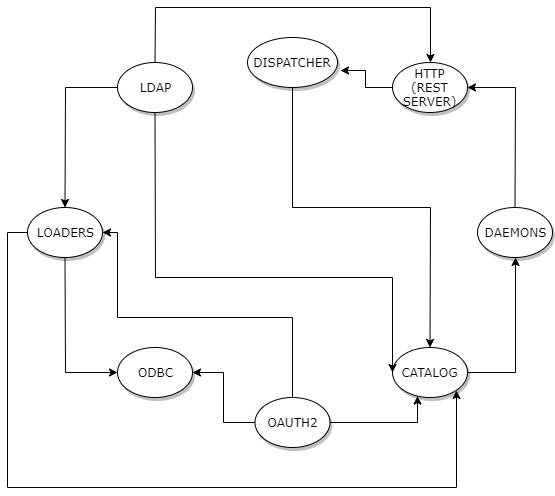
\includegraphics[scale = 0.70]{img/ResourcesEMS.png}
	\caption{Mapeamento dos recursos do barramento de serviços.}
	\label{fun:fig:ResourcesEMS}
	\end{center}
\end{figure}





%Com a implementação de serviços para gerar as informações do monitoramento, necessita-se definir um padrão ou \textit{design} para a realização da coleta, armazenamento e analise dos dados do monitoramento. Esse trabalho propõe a implementação de serviços para a realização da coleta, o desenho de um modelo de dados para o armazenamento dos dados monitorados e \textit{web services} para realização de integração com qualquer ferramenta que utilize o protocolo SNMP afim de fornecer informações para uma linguagem que permita facilmente o entendimento humano. %

%\\\\\\\\\\\\\\\\\\\\\\\\\\\\\\\\\\\\\\\\\\\\\\\\

\subsection{Desempenho}

Na literatura durante a realização da pesquisa percebeu-se a identificação de um item preocupante em relação as informações monitoradas, esse item é o desempenho, devido à quantidade de informações geradas durante o monitoramento. O trabalho tem como proposta a realização do armazenamento das informações sem problemas de desempenho, com a otimização das consultas dos serviços responsáveis pela realização e geração das informações geradas pelo monitoramento.       

%\\\\\\\\\\\\\\\\\\\\\\\\\\\\\\\\\\\\\\\\\\\\\\\\


\section{Instrumenção de código}

Este trabalho será desenvolvido por meio de seis tarefas listadas a seguir durante os períodos 2018/2 e 2019/1 que são registrados oficialmente no calendário acadêmico da UnB, e por meio do cronograma apresentado na Tabela \ref{tab:cronograma}.

	1. Escolha das abordagens que serão utilizadas por meio de características não exploradas nas soluções atuais de Implementação do protocolo SNMP para monitoramento de serviços;
  
  2. Desenvolvimento de novas abordagens que serão utilizadas na Implementação do protocolo SNMP para monitoramento de serviços ;
    
  3. Prova de conceito das abordagens desenvolvidas;
    
  4. Escrita de artigos científicos para a de submissão em congressos e periódicos;
  
  5. Escrita da dissertação de mestrado;
  
  6. Defesa do mestrado.

\begin{table}[!htpb]
	\centering
	\caption{Cronograma de execução de atividades}
	\begin{center}
		\begin{tabular}{|l|c|c|c|c|c|c|c|c|c|c|c|c|c|} \hline
Tarefa&ABR&MAI&JUN&JUL&AGO&SET&OUT&NOV&DEZ\\
			\hline
			Tarefa 1 &X&X&X& & & & & & \\
			\hline
			Tarefa 2 & & & &X&X&X& & & \\
			\hline
			Tarefa 3 & & & & &X&X&X& & \\
			\hline
			Tarefa 4 & & & & &X&X&X& & \\
			\hline
			Tarefa 5 & & & &&X&X&X&X&X \\
			\hline
			Tarefa 6 & & & & & & & & X& \\
			\hline
		\end{tabular}
		\label{tab:cronograma}
	\end{center}
\end{table} 


\fontshape{n}\selectfont%